\documentclass{article}

\usepackage{arxiv}

\usepackage[utf8]{inputenc} % allow utf-8 input
\usepackage[T1]{fontenc}    % use 8-bit T1 fonts
\usepackage{lmodern}        % https://github.com/rstudio/rticles/issues/343
\usepackage{hyperref}       % hyperlinks
\usepackage{url}            % simple URL typesetting
\usepackage{booktabs}       % professional-quality tables
\usepackage{amsfonts}       % blackboard math symbols
\usepackage{nicefrac}       % compact symbols for 1/2, etc.
\usepackage{microtype}      % microtypography
\usepackage{graphicx}

\title{senatebR: coletando dados do Senado Federal brasileiro}

\author{
    Vinicius Santos
    \thanks{Doutor em Ciência Política (UFMG). Exerce o cargo de
Cientista de Dados e presta Assessoria Parlamentar CTI / IA no Senado
Federal - Brasília. Atuou em Pesquisas de Mercado/Notas Técnicas para
Consultorias, Terceiro Setor e Governo. \url{http://vsantos.rbind.io/}}
   \\
    Núcleo de Dados - GLPT/SF \\
    Senado Federal \\
  Brasília, DF \\
  \texttt{\href{mailto:santos.vinicius18@gmail.com}{\nolinkurl{santos.vinicius18@gmail.com}}} \\
  }

% Pandoc syntax highlighting
\usepackage{color}
\usepackage{fancyvrb}
\newcommand{\VerbBar}{|}
\newcommand{\VERB}{\Verb[commandchars=\\\{\}]}
\DefineVerbatimEnvironment{Highlighting}{Verbatim}{commandchars=\\\{\}}
% Add ',fontsize=\small' for more characters per line
\usepackage{framed}
\definecolor{shadecolor}{RGB}{248,248,248}
\newenvironment{Shaded}{\begin{snugshade}}{\end{snugshade}}
\newcommand{\AlertTok}[1]{\textcolor[rgb]{0.94,0.16,0.16}{#1}}
\newcommand{\AnnotationTok}[1]{\textcolor[rgb]{0.56,0.35,0.01}{\textbf{\textit{#1}}}}
\newcommand{\AttributeTok}[1]{\textcolor[rgb]{0.13,0.29,0.53}{#1}}
\newcommand{\BaseNTok}[1]{\textcolor[rgb]{0.00,0.00,0.81}{#1}}
\newcommand{\BuiltInTok}[1]{#1}
\newcommand{\CharTok}[1]{\textcolor[rgb]{0.31,0.60,0.02}{#1}}
\newcommand{\CommentTok}[1]{\textcolor[rgb]{0.56,0.35,0.01}{\textit{#1}}}
\newcommand{\CommentVarTok}[1]{\textcolor[rgb]{0.56,0.35,0.01}{\textbf{\textit{#1}}}}
\newcommand{\ConstantTok}[1]{\textcolor[rgb]{0.56,0.35,0.01}{#1}}
\newcommand{\ControlFlowTok}[1]{\textcolor[rgb]{0.13,0.29,0.53}{\textbf{#1}}}
\newcommand{\DataTypeTok}[1]{\textcolor[rgb]{0.13,0.29,0.53}{#1}}
\newcommand{\DecValTok}[1]{\textcolor[rgb]{0.00,0.00,0.81}{#1}}
\newcommand{\DocumentationTok}[1]{\textcolor[rgb]{0.56,0.35,0.01}{\textbf{\textit{#1}}}}
\newcommand{\ErrorTok}[1]{\textcolor[rgb]{0.64,0.00,0.00}{\textbf{#1}}}
\newcommand{\ExtensionTok}[1]{#1}
\newcommand{\FloatTok}[1]{\textcolor[rgb]{0.00,0.00,0.81}{#1}}
\newcommand{\FunctionTok}[1]{\textcolor[rgb]{0.13,0.29,0.53}{\textbf{#1}}}
\newcommand{\ImportTok}[1]{#1}
\newcommand{\InformationTok}[1]{\textcolor[rgb]{0.56,0.35,0.01}{\textbf{\textit{#1}}}}
\newcommand{\KeywordTok}[1]{\textcolor[rgb]{0.13,0.29,0.53}{\textbf{#1}}}
\newcommand{\NormalTok}[1]{#1}
\newcommand{\OperatorTok}[1]{\textcolor[rgb]{0.81,0.36,0.00}{\textbf{#1}}}
\newcommand{\OtherTok}[1]{\textcolor[rgb]{0.56,0.35,0.01}{#1}}
\newcommand{\PreprocessorTok}[1]{\textcolor[rgb]{0.56,0.35,0.01}{\textit{#1}}}
\newcommand{\RegionMarkerTok}[1]{#1}
\newcommand{\SpecialCharTok}[1]{\textcolor[rgb]{0.81,0.36,0.00}{\textbf{#1}}}
\newcommand{\SpecialStringTok}[1]{\textcolor[rgb]{0.31,0.60,0.02}{#1}}
\newcommand{\StringTok}[1]{\textcolor[rgb]{0.31,0.60,0.02}{#1}}
\newcommand{\VariableTok}[1]{\textcolor[rgb]{0.00,0.00,0.00}{#1}}
\newcommand{\VerbatimStringTok}[1]{\textcolor[rgb]{0.31,0.60,0.02}{#1}}
\newcommand{\WarningTok}[1]{\textcolor[rgb]{0.56,0.35,0.01}{\textbf{\textit{#1}}}}

% tightlist command for lists without linebreak
\providecommand{\tightlist}{%
  \setlength{\itemsep}{0pt}\setlength{\parskip}{0pt}}



\begin{document}
\maketitle


\begin{abstract}
Este artigo cumopre o objetivo de introduzir um novo pacote em linguagem
R criado com o propósito de simplificar a interação com as APIs bem como
na obtenção de dados por meio de web scraping do Senado
Federal/Congresso Nacional. O objetivo central é disponibilizar à
comunidade acadêmica uma ferramenta que permita o acesso eficiente a
dados legislativos. A proposta é acompanhada por uma nota técnica que
detalha a implementação do pacote, seu escopo e a metodologia empregada
assim como estudos de caso elucidando seu potencial de uso. Assim, a
iniciativa visa facilitar o processo de pesquisa e análise para
estudiosos e profissionais interessados no acompanhamento das atividades
legislativas do Senado Federal brasileiro.
\end{abstract}

\keywords{
    programação
   \and
    ciência de dados
   \and
    API
   \and
    senado federal
  }

Title (English): senatebR: collecting data from the Brazilian Federal
Senate

Abstract (English): This article introduces a new R language package
created with the aim of simplifying interaction with APIs and obtaining
data via the web scraping site of the Federal Senate / National
Congress. The main objective is to provide the academic community with a
tool that allows efficient access to legislative data. The proposal is
accompanied by a technical note detailing the implementation of the
package, its scope and the methodology employed and case studies
elucidating its potential use. Thus, the initiative aims to facilitate
the research and analysis process for scholars and professionals
interested in monitoring the legislative activities of the Brazilian
Federal Senate.

Keywords: programming, data science, API, webscraping, federal senate

Authors' contribution statement: The authors state to have equally
participatedin the conception, elaboration and revision of the final
version of this article.

Conflict of interests statement: The authors declare no conflict of
interests.

\section{Introduction}\label{introduction}

No debate sobre governo aberto, a disponibilidade de dados é vista como
um basilar para o funcionamento transparente e eficaz de qualquer
democracia (Yu e Robinson, 2012; Francoli e Clarke, 2014;
Sandoval-Almazan e Gil-Garcia, 2014; Abu-Shanab, 2015; De Blasio e
Sorice, 2016; Kornberger et al, 2017). No caso do senado brasileiro,
esses dados não apenas fornecem insights sobre o processo legislativo,
mas também permitem a análise das políticas públicas a serem postas em
ação, bem como do comportamento dos legisladores. Diante disso, o acesso
aos dados do Senado Federal desempenha, portanto, papel fundamental na
medida em que pode oferecer um conjunto de informações sobre as
atividades legislativas do país (Gherghina e Katsanidou, 2013; Lupia e
Elman, 2014; Gleditsch e Janz, 2016; Stockemer, Koehler e Lenz, 2018).

A motivação por trás do desenvolvimento do pacote \emph{senatebR}, assim
como iniciativas similares (Meireles, Silva e Costa, 2016; Mcdonnell,
Duarte e Freire, 2019; Morais, 202; Saldanha, Bastos e Barcellos, 2019;
Meireles e Torres, 2021), esteve ancorada na necessidade de tornar as
informações da Câmara Alta acessíveis e de fácil utilização para a
comunidade acadêmica, para consultores ou para qualquer pessoa
interessada em compreender e analisar, no nosso caso, o cenário político
brasileiro. Disso decorre que, a capacidade de acessar e analisar dados
legislativos de maneira eficiente não apenas enriquece o debate público,
mas também fortalece a participação cívica e a prestação de contas no
sistema democrático (Gherghina e Katsanidou, 2013).

O Senado Federal brasileiro, como uma das casas do Congresso Nacional,
desempenha um papel significativo na elaboração e revisão de leis e
políticas públicas (Rubiatti, 2017, 2020). Portanto, seus procedimentos,
debates e decisões são de central interesse para pesquisadores,
acadêmicos, jornalistas, consultores e cidadãos preocupados com questões
políticas, sociais e econômicas. Ao destacar a relevância do Senado
Federal como fonte de dados para análises, reconhecemos a importância de
garantir que essas informações estejam disponíveis e sejam facilmente
acessíveis para todos os interessados.

Diante disso, as pesquisas podem se beneficiar do acesso facilitado aos
dados legislativos, eliminando, por conseguinte, a necessidade de coleta
manual de informações. Ademais, o pacote fornece a possibilidade de, ao
reduzir o custo de tempo do acesso à informação, os cientistas possam
dedicar maior tempo e consequentemente concentrar sua atenção na análise
e visualizar dados, permitindo, portanto, que os pesquisadores conduzam
estudos de maior profundidade.

\section{Escopo e propósito do pacote: acesso aos dados e
reprodutibilidade}\label{escopo-e-propuxf3sito-do-pacote-acesso-aos-dados-e-reprodutibilidade}

A reprodutibilidade é um princípio fundamental na pesquisa acadêmica,
pois garante que os resultados obtidos possam ser verificados, validados
e reproduzidos por outros pesquisadores. Isso não apenas promove
transparência e confiança na pesquisa, como também permite que avanços
científicos sejam construídos sobre bases sólidas e confiáveis . Nesse
contexto, a reprodutibilidade desempenha um papel fundamental na
validação e no avanço do conhecimento científico. Permite que outros
pesquisadores verifiquem os resultados de estudos anteriores, testem
hipóteses alternativas e construam sobre o trabalho existente.
(Christensen e Soderberg, 2015; Da-Rt, 2012; Elman e Kapiszewski, 2014;
Dunning e Rosenblatt, 2016; Freese e Peterson, 2017; Figueiredo Filho,
et al, 2019).

Além disso, promove a transparência e a integridade na pesquisa,
ajudando a evitar erros, vieses e má conduta científica. Portanto,
garantir a reprodutibilidade dos resultados é essencial para a
confiabilidade e credibilidade da pesquisa acadêmica (Gherghina e
Katsanidou, 2013; Lupia e Elman, 2014; Gleditsch e Janz, 2016;
Stockemer, Koehler e Lenz, 2018; Figueiredo Filho, et al, 2019).

O pacote \emph{senatebR} foi projetado com foco na reprodutibilidade,
facilitando a replicação dos resultados obtidos e a realização de
análises comparativas por outros pesquisadores. Para demonstrar a
reprodutibilidade, o código-fonte do pacote é estruturado de forma clara
e organizada, seguindo as melhores práticas de programação e
documentação\footnote{Consultar site do projeto:
  \url{https://vsntos.github.io/senatebR/}}. Todas as funções e métodos
são acompanhados por documentação ampla, explicando seu propósito,
parâmetros e exemplos de uso. Isso permite que outros pesquisadores
entendam de forma facilitada como utilizar o pacote e reproduzir os
resultados (Wickham, Bryan, 2023).** As principais funcionalidades do
pacote incluem:

\begin{enumerate}
\def\labelenumi{\Roman{enumi})}
\item
  Acesso à API do Senado Federal: o pacote permite a interação direta
  com a API do Senado Federal, facilitando a obtenção de dados
  atualizados sobre projetos de lei, tramitações legislativas, votações,
  comissões, parlamentares e outras informações.
\item
  Obtenção de Dados por Web Scraping: além da API, o pacote também
  incorpora funcionalidades de web scraping para extrair dados
  diretamente do site do Senado Federal e/ou sítio eletrônico do
  Congresso Nacional, garantindo acesso abrangente a informações
  legislativas mesmo quando não estão disponíveis ou o acesso de outras
  informações oferecidas pela API.
\end{enumerate}

Assim, foi desenvolvido para abranger uma ampla gama de funcionalidades
visando atender às necessidades dos pesquisadores acadêmicos e de
qualquer pessoa interessada em análises legislativas detalhadas. Este
pacote oferece dados detalhados em cinco dimensões principais:

\begin{enumerate}
\def\labelenumi{\arabic{enumi})}
\item
  Projetos e Matérias: Este conjunto de dados permite identificar e
  acompanhar projetos de lei, propostas legislativas e outras matérias
  em tramitação no Senado Federal. Com isso, o usuário tem acesso a
  detalhes como título, emenda, autor, status atual e histórico de
  tramitação.
\item
  Informações sobre Parlamentares: nesse módulo, os utilizadores podem
  explorar perfis de atuais e antigos parlamentares do Senado Federal,
  incluindo biografias, filiações partidárias, história legislativa,
  entre outras informações relevantes.
\item
  Informações sobre a composição: este módulo oferece uma visão geral da
  composição atual do Senado Federal, incluindo a distribuição
  partidária dos senadores, as suas unidades federativas de origem, a
  duração do mandato, bem como dados demográficos e estatísticas
  relevantes.
\item
  Informações sobre as comissões: aqui, os usuários podem ter acesso a
  detalhes sobre as diferentes comissões do Senado Federal, incluindo as
  suas funções, membros atuais, agendas de trabalho e outras atividades
  relacionadas.
\item
  Informações sobre o Plenário: este último componente fornece
  informações sobre as atividades do plenário do Senado Federal,
  incluindo pautas de votação, transcrições de debates, vetos, medidas
  provisórias, decisões tomadas e outras informações relevantes.
\end{enumerate}

Portanto, entre suas potencialidades de uso estão:

\begin{enumerate}
\def\labelenumi{\arabic{enumi})}
\item
  Análise de Dados Legislativos: uma vez que o usuário tenha
  familiaridade com ferramentas para limpeza, manipulação e análise de
  dados, o pacote permite que os usuários realizem uma ampla variedade
  de análises legislativas, incluindo tendências legislativas ao longo
  do tempo, padrões de votação, padrões de participação em comissões,
  entre outros.
\item
  Visualização de Dados: o pacote oferece a possibilidade de com
  mobilização de recursos adicionais os usuários possam visualizar os
  dados por meios de gráficos, mapas e outras representações visuais dos
  dados legislativos, tornando as análises mais acessíveis e
  compreensíveis.
\end{enumerate}

Como dito até aqui, o \emph{senatebR} abrange uma variedade de dados do
Senado Federal, incluindo informações sobre projetos de lei, autores,
tramitações, votações, comissões, parlamentares, partidos políticos,
entre outros. Essa abrangência de dados permite que os usuários realizem
análises multifacetadas e detalhadas do processo legislativo brasileiro
facilitando pesquisas, por exemplo, de perfis parlamentares (Lemos e
Ranincheski, 2008), composição e dinâmica das comissões (Nascimento,
2012; Souza e Silva, 2019; Ferreira e Rubiatti, 2022; Santos e Belém
Lopes, 2022; Santos, 2024) assim como de produção legislativa (Ricci,
2008; Oliveira, 2019).

O pacote inclui uma variedade de métodos e funções para realizar
diferentes tarefas relacionadas à coleta, para posterior processamento e
análise de dados legislativos. Entre as principais funções temos:

\begin{enumerate}
\def\labelenumi{\arabic{enumi}.}
\tightlist
\item
  Coleta dos dados sobre os senadores por Legislatura
\end{enumerate}

A função recebe como argumento o ano da legislatura de início dos dados
que se busca é a legislatura de fim do intervalo desejado. O código
abaixo permite, portanto, a coleta de dados das legislaturas no
intervalo entre a 47 e 56.

\begin{Shaded}
\begin{Highlighting}[]
\FunctionTok{library}\NormalTok{(senatebR)}
\end{Highlighting}
\end{Shaded}

\begin{Shaded}
\begin{Highlighting}[]
\NormalTok{df\_senadores\_legislatura }\OtherTok{\textless{}{-}} \FunctionTok{obter\_dados\_senadores\_legislatura}\NormalTok{(}\DecValTok{47}\NormalTok{, }\DecValTok{56}\NormalTok{)}

\FunctionTok{glimpse}\NormalTok{(df\_senadores\_legislatura)}
\end{Highlighting}
\end{Shaded}

\begin{verbatim}
## Rows: 929
## Columns: 13
## $ IdentificacaoParlamentar.CodigoParlamentar       <chr> "4865", "168", "5573"~
## $ IdentificacaoParlamentar.NomeParlamentar         <chr> "Abdala Karin Nabut",~
## $ IdentificacaoParlamentar.NomeCompletoParlamentar <chr> "Abdala Karin Nabut",~
## $ IdentificacaoParlamentar.SexoParlamentar         <chr> "Masculino", "Masculi~
## $ IdentificacaoParlamentar.FormaTratamento         <chr> "Senador ", "Senador ~
## $ IdentificacaoParlamentar.UrlFotoParlamentar      <chr> NA, "http://www.senad~
## $ IdentificacaoParlamentar.UrlPaginaParlamentar    <chr> NA, "http://www25.sen~
## $ IdentificacaoParlamentar.SiglaPartidoParlamentar <chr> NA, NA, "PDT", "CIDAD~
## $ IdentificacaoParlamentar.CodigoPublicoNaLegAtual <chr> NA, NA, NA, NA, "916"~
## $ IdentificacaoParlamentar.UrlPaginaParticular     <chr> NA, NA, NA, NA, "http~
## $ IdentificacaoParlamentar.EmailParlamentar        <chr> NA, NA, NA, NA, "sen.~
## $ IdentificacaoParlamentar.UfParlamentar           <chr> NA, NA, NA, NA, NA, N~
## $ Mandatos.Mandato                                 <list> ["246", "DF", ["52",~
\end{verbatim}

Com isso, uma vez seguidos esses passos, a função retorna uma base de
dados de 929 observações e 12 variáveis\footnote{Disponível em:}.

\begin{enumerate}
\def\labelenumi{\arabic{enumi}.}
\setcounter{enumi}{1}
\tightlist
\item
  Coleta dos dados sobre Medidas Provisórias
\end{enumerate}

Para esse conjunto de dados, o pacote oferece duas opções: i) a coleta
dos dados das MPs em tramitação e os dados das MPs encerradas. Sendo
assim, a função a coleta feita no dia 12/06/2024 gerou um \emph{data
frame} de 24 observações e 5 (cinco) variáveis (mpv\_em\_tramitacao
\textless- coletar\_medidas\_provisorias\_em\_tramitacao()).

\begin{Shaded}
\begin{Highlighting}[]
\NormalTok{mpv\_em\_tramitacao }\OtherTok{\textless{}{-}} \FunctionTok{coletar\_medidas\_provisorias\_em\_tramitacao}\NormalTok{()}

\FunctionTok{glimpse}\NormalTok{(mpv\_em\_tramitacao)}
\end{Highlighting}
\end{Shaded}

\begin{verbatim}
## Rows: 24
## Columns: 5
## $ Link    <chr> "https://www.congressonacional.leg.br/materias/medidas-proviso~
## $ Matéria <chr> "MPV 1232/2024", "MPV 1231/2024", "MPV 1230/2024", "MPV 1229/2~
## $ Ementa  <chr> "Altera a Lei nº 12.111, de 9 de dezembro de 2009, que dispõe ~
## $ Prazo   <chr> "25/08/2024 - NA", "24/08/2024 - NA", "19/08/2024 - NA", "19/0~
## $ Status  <chr> "em tramitação", "em tramitação", "em tramitação", "em tramita~
\end{verbatim}

Já as medidas provisórias encerradas (coleta feita no mesmo dia com
todas as páginas) totalizam 7268 observações e seis variáveis
(mpv\_encerradas \textless-
coletar\_medidas\_provisorias\_encerradas(364)).

\begin{Shaded}
\begin{Highlighting}[]
\NormalTok{mpv\_encerradas }\OtherTok{\textless{}{-}} \FunctionTok{coletar\_medidas\_provisorias\_encerradas}\NormalTok{(}\DecValTok{364}\NormalTok{)}
\FunctionTok{glimpse}\NormalTok{(mpv\_encerradas)}
\end{Highlighting}
\end{Shaded}

\begin{verbatim}
## Rows: 7,270
## Columns: 6
## $ Link             <chr> "https://www.congressonacional.leg.br/materias/medida~
## $ MPV              <chr> " MPV 1218/2024 ", " MPV 1210/2024 ", " MPV 1206/2024~
## $ Título           <chr> NA, NA, NA, NA, NA, NA, NA, NA, NA, NA, NA, NA, NA, N~
## $ Ementa           <chr> "Abre crédito extraordinário, em favor de diversos ór~
## $ Prazo.de.60.dias <chr> "09/07/2024", "18/05/2024", "05/04/2024", "01/04/2024~
## $ Prazo.de.emendas <chr> "Encerrado", "Encerrado", "Encerrado", "Encerrado", "~
\end{verbatim}

\begin{enumerate}
\def\labelenumi{\arabic{enumi}.}
\setcounter{enumi}{2}
\tightlist
\item
  Coleta de dados de Vetos com tramitação encerrada
\end{enumerate}

Por fim, para cumprir com a tarefa inicial de apresentar exemplos que
indiquem as potencialidades do pacote, é possível coletar também dados
referentes aos vetos com sua tramitação encerrada (dados\_vetos
\textless- info\_vetos(pages = 20)) somam 987 observações e 6 (seis)
variáveis.

\begin{Shaded}
\begin{Highlighting}[]
\NormalTok{dados\_vetos }\OtherTok{\textless{}{-}} \FunctionTok{info\_vetos}\NormalTok{(}\AttributeTok{pages =} \DecValTok{20}\NormalTok{)}
\FunctionTok{glimpse}\NormalTok{(dados\_vetos)}
\end{Highlighting}
\end{Shaded}

\begin{verbatim}
## Rows: 987
## Columns: 6
## $ Veto           <chr> "VET 11/2024 - Parcial", "VET 8/2024 - Parcial", "VET 7~
## $ Link           <chr> "https://www.congressonacional.leg.br/materias/vetos/-/~
## $ Ementa         <chr> "Veto Parcial aposto ao Projeto de Lei Complementar nº ~
## $ Sobresta       <chr> "16/06/2024", "12/05/2024", "12/05/2024", "09/05/2024",~
## $ Materia_Vetada <chr> "PLP 233/2023", "PL 2253/2022", "PL 6379/2019", "PL 565~
## $ Norma_Gerada   <chr> "Lei Complementar nº 207 de 16/05/2024", "Lei nº 14.843~
\end{verbatim}

Assim, feita essa introdução, passaremos para a apresentação de um
estudo de caso que demonstra o fluxo de trabalho de análise utilizando o
pacote de coleta de dados do Senado Federal. Este estudo de caso oferece
uma visão prática de como aplicar efetivamente o pacote em pesquisas
acadêmicas e projetos de análise legislativa.

\textbf{2.1. Estudo de Caso: Pronunciamento dos Parlamentares}

Antes de abordarmos propriamente o estudo de caso, cabe retomar o ciclo
do dado pelo qual atravessa um cientista. Dito isso, é importante
retomar o modelo das etapas de um projeto típico de ciência de dados
proposto por Wickham, Çetinkaya-Rundel e Grolemund (2023). O fluxo de
trabalho para os autores consideram como primeiro passo a i) importação
de dados é seguido da ii) limpeza e organização, que continuaria seu
percurso na iii) transformação das informações, até chegar na iv)
visualização e modelagem, para, por fim, permitir que sejam comunicados
os resultados (Wickham, Çetinkaya-Rundel e Grolemund, 2023).

Na ingestão de dados, as informações são importadas para o ambiente de
análise, geralmente em um formato de banco de dados e carregados, no
nosso caso, na linguagem de programação R. Em seguida, é na limpeza e
organização dos dados (\emph{tidying}) que organizamos as informações de
forma consistente, nesse caso, cada coluna representaria uma variável e
cada linha uma observação (Wickham, Çetinkaya-Rundel e Grolemund, 2023).

Na transformação dos dados (também chamada de \emph{wrangling}) nos
concentramos, por exemplo, na criação de novas variáveis a partir de
variáveis existentes e no cálculo estatísticas de resumo. Assim, fica
reservado a etapa de visualização a tarefa de revelar insights e
levantar novas questões, enquanto na modelagem espera-se não só a
extração de informações relevantes como, dependendo do objetivo da
pesquisa, entre outras tarefas, prever resultados. Por fim, cabe aos
cientistas a tarefa de transmitir de forma clara e eficaz as descobertas
obtidas durante a análise de dados (Wickham, Çetinkaya-Rundel e
Grolemund, 2023).

Com base nesse quadro de referência, seguiremos com nosso estudo de
caso. Para a coleta retornaremos a operação de coleta de dados dos
parlamentares apresentada na seção anterior. Usaremos essa base de dados
como referência. Nesse caso, optamos, para esse exercício, coletar
informações dos pronunciamentos dos senadores apenas da 56ª legislatura.
Veja o exemplo a seguir:

\begin{Shaded}
\begin{Highlighting}[]
\NormalTok{df\_senadores\_legislatura\_56 }\OtherTok{\textless{}{-}} \FunctionTok{obter\_dados\_senadores\_legislatura}\NormalTok{(}\DecValTok{56}\NormalTok{, }\DecValTok{56}\NormalTok{)}
\end{Highlighting}
\end{Shaded}

\begin{verbatim}
## No encoding supplied: defaulting to UTF-8.
\end{verbatim}

\begin{Shaded}
\begin{Highlighting}[]
\FunctionTok{glimpse}\NormalTok{(df\_senadores\_legislatura\_56)}
\end{Highlighting}
\end{Shaded}

\begin{verbatim}
## Rows: 245
## Columns: 13
## $ IdentificacaoParlamentar.CodigoParlamentar       <chr> "5573", "4981", "5918~
## $ IdentificacaoParlamentar.NomeParlamentar         <chr> "Abel Rebouças", "Aci~
## $ IdentificacaoParlamentar.NomeCompletoParlamentar <chr> "Abel Rebouças São Jo~
## $ IdentificacaoParlamentar.SexoParlamentar         <chr> "Masculino", "Masculi~
## $ IdentificacaoParlamentar.FormaTratamento         <chr> "Senador ", "Senador ~
## $ IdentificacaoParlamentar.SiglaPartidoParlamentar <chr> "PDT", "PDT", NA, "PE~
## $ IdentificacaoParlamentar.CodigoPublicoNaLegAtual <chr> NA, "916", NA, NA, NA~
## $ IdentificacaoParlamentar.UrlFotoParlamentar      <chr> NA, "http://www.senad~
## $ IdentificacaoParlamentar.UrlPaginaParlamentar    <chr> NA, "http://www25.sen~
## $ IdentificacaoParlamentar.UrlPaginaParticular     <chr> NA, "https://acirgurg~
## $ IdentificacaoParlamentar.EmailParlamentar        <chr> NA, "sen.acirgurgacz@~
## $ IdentificacaoParlamentar.UfParlamentar           <chr> NA, NA, NA, NA, NA, N~
## $ Mandatos.Mandato                                 <list> ["492", "BA", ["55",~
\end{verbatim}

Com a operação anterior, obtivemos uma base de dados composta por 245
observações e 13 variáveis. Dessa base de dados utilizaremos o vetor
df\_senadores\_legislatura56\$IdentificacaoParlamentar.CodigoParlamentar*
para utitilizar na função
extrair\_pronunciamentos\_multi(codigos\_parlamentares, anos). Com essa
função conseguimos acessar todos os pronunciamentos num intervalo de
tempo determinado. Veja a função abaixo:

\begin{Shaded}
\begin{Highlighting}[]
\NormalTok{dados\_multi }\OtherTok{\textless{}{-}} \FunctionTok{extrair\_pronunciamentos\_multi}\NormalTok{(}\AttributeTok{codigos\_parlamentares =} 
\NormalTok{                                               df\_senadores\_legislatura\_56}\SpecialCharTok{$}\NormalTok{IdentificacaoParlamentar.CodigoParlamentar, }\AttributeTok{anos =} \FunctionTok{c}\NormalTok{(}\DecValTok{2020}\SpecialCharTok{:}\DecValTok{2024}\NormalTok{))}
\end{Highlighting}
\end{Shaded}

Dito de outra forma, o que estamos buscando, portanto, por meio da
função anterior, são as informações de todos os pronunciamentos de todos
os senadores da 56ª legislatura entre 2020 e 2024. O código gera uma
base de dados composta por 3210 observações e 8 variáveis.

\begin{Shaded}
\begin{Highlighting}[]
\FunctionTok{glimpse}\NormalTok{(dados\_multi)}
\end{Highlighting}
\end{Shaded}

\begin{verbatim}
## Rows: 3,210
## Columns: 8
## $ Codigo_Parlamentar    <chr> "4981", "4981", "4981", "4981", "4981", "4981", ~
## $ Ano                   <int> 2020, 2020, 2020, 2020, 2020, 2020, 2020, 2020, ~
## $ Data_Pronunciamento   <chr> "15/12/2020", "13/08/2020", "05/08/2020", "30/07~
## $ Tipo_Pronunciamento   <chr> "Discurso", "Discurso", "Discurso", "Discurso", ~
## $ Casa                  <chr> "Senado Federal", "Senado Federal", "Senado Fede~
## $ Partido_UF            <chr> "PDT/RO", "PDT/RO", "PDT/RO", "PDT/RO", "PDT/RO"~
## $ Resumo_Pronunciamento <chr> "Elogios ao Presidente do Senado, Davi Alcolumbr~
## $ Link_Pronunciamento   <chr> "https://www25.senado.leg.br/web/atividade/pronu~
\end{verbatim}

Seguiremos então para a etapa de transformação dos dados. Perceba que a
variável: dados\_multi\$Partido\_UF{[}1{]} apresenta as informações do
partido e da unidade federativa da seguinte maneira: {[}1{]} ``PDT/RO''.
Para aqueles leitores já iniciados em programação/ciência de dados
podemos, portanto, separar cada uma das informações em variáveis
distintas por meio da seguinte operação:

\begin{Shaded}
\begin{Highlighting}[]
\NormalTok{dados\_multi }\OtherTok{\textless{}{-}}\NormalTok{ dados\_multi }\SpecialCharTok{\%\textgreater{}\%} 
                  \FunctionTok{separate}\NormalTok{(Partido\_UF, }\AttributeTok{into =} \FunctionTok{c}\NormalTok{(}\StringTok{"Partido"}\NormalTok{, }\StringTok{"UF"}\NormalTok{), }\AttributeTok{sep =} \StringTok{"/"}\NormalTok{)}
\end{Highlighting}
\end{Shaded}

Em outras palavras, o que estamos fazendo com essa função é separar em
duas colunas (``Partido'', ``UF'') a informação de Partido\_UF tendo
como referência o separador ``/''. Com esse procedimento temos na base
de dados uma variável para Partido e outra para UF fazendo com que a
base de dados tenha agora 9 variáveis.

Os resultados da análise podem ser visualizados em gráficos, tabelas e
outros tipos de representações visuais para facilitar a interpretação e
comunicação dos resultados. Isso permite que o pesquisador identifique
padrões e tendências de forma mais clara e compreensível. Veja o
conjunto de exemplos abaixo em que apresentamos um conjunto de
estatísticas descritivas para a base de dados coletada no passo anterior
(dados\_multi).

Abaixo apresentamos os dados sobre a frequência dos discursos por ano.
Como é possível depreender, no intervalo entre os anos de 2020 e 2024,
2022 com 810 discursos se destacou como aquele ano em que os senadores
mais se dispuserem a expor seus pontos de vista no Senado.

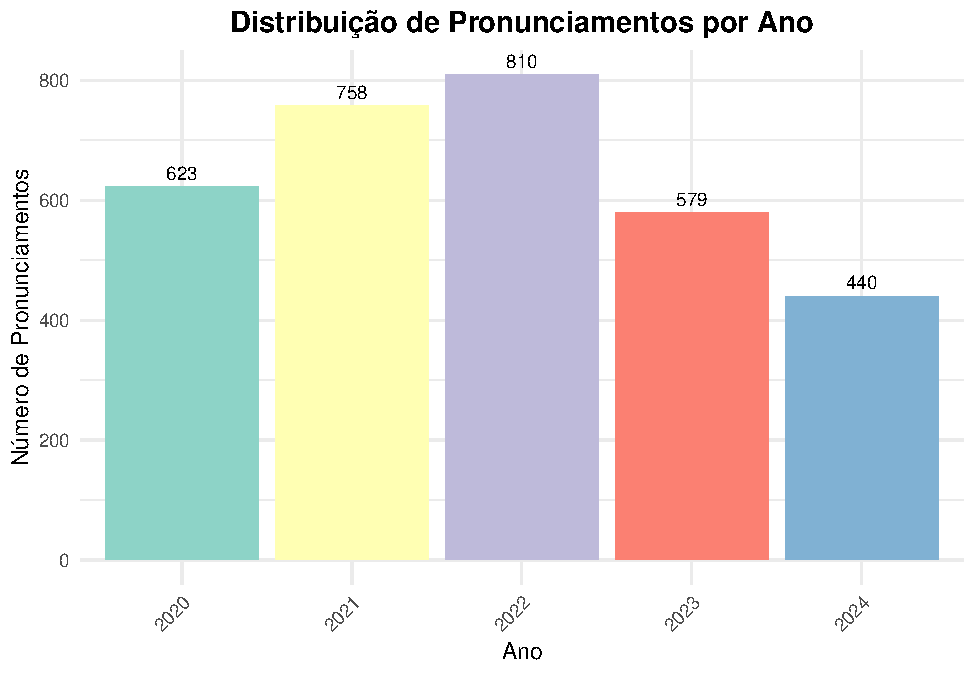
\includegraphics{Texto_files/figure-latex/unnamed-chunk-11-1.pdf}

No gráfico a seguir seguimos observando a distribuição dos discursos no
tempo. Porém, nessa variação apresentamos essa frequência em termos
mensais. O que os dados sugerem é que os meses que antecedem o recesso
parlamentar, quais sejam, junho e julho assim como novembro e dezembro,
são os que concentram maior exposição dos parlamentares observados.

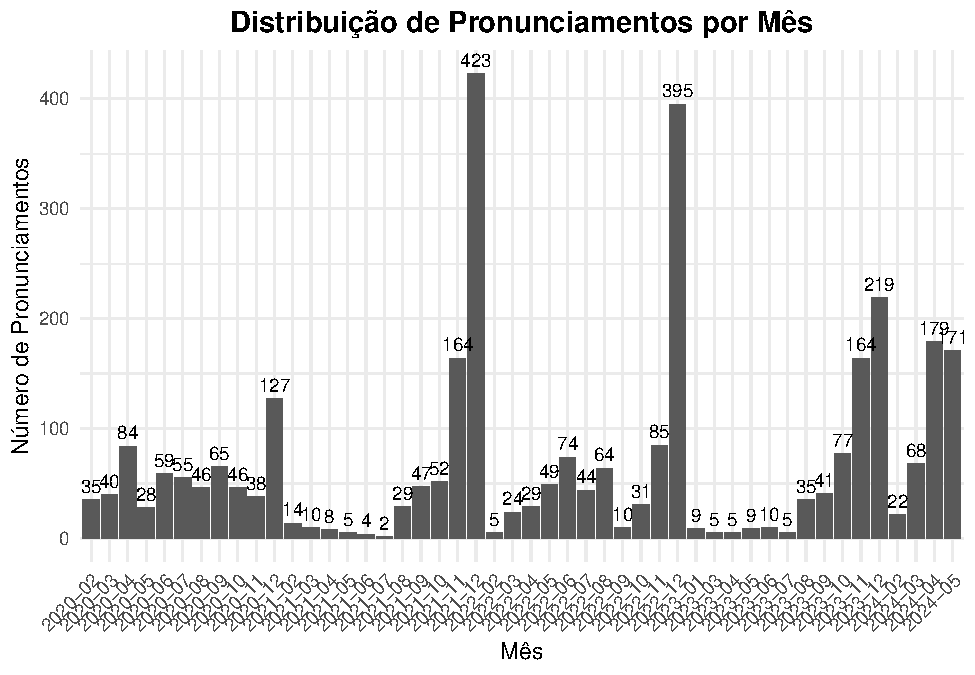
\includegraphics{Texto_files/figure-latex/unnamed-chunk-12-1.pdf}

Seguimos nosso exercício descritivo observado os pronunciamentos por
tipo. Os dados permitem observar, como esperado, que o uso da palavra se
concentra nos discursos. No entanto, cabe observar que esse tipo de uso
da palavra é seguido por pronunciamentos ``Pela Ordem'', seguido dos
dedicados a ``Orientação à bancada'' e o uso da palavra para
``Discussão'' é o quarto motivo pelo qual o uso do microfone é
mobilizado. Por fim, os tipos de pronunciamentos que fecham o cinco
principais motivos de uso da palavra é aquela feito pelo relator, seja
para proferir parecer ou não.

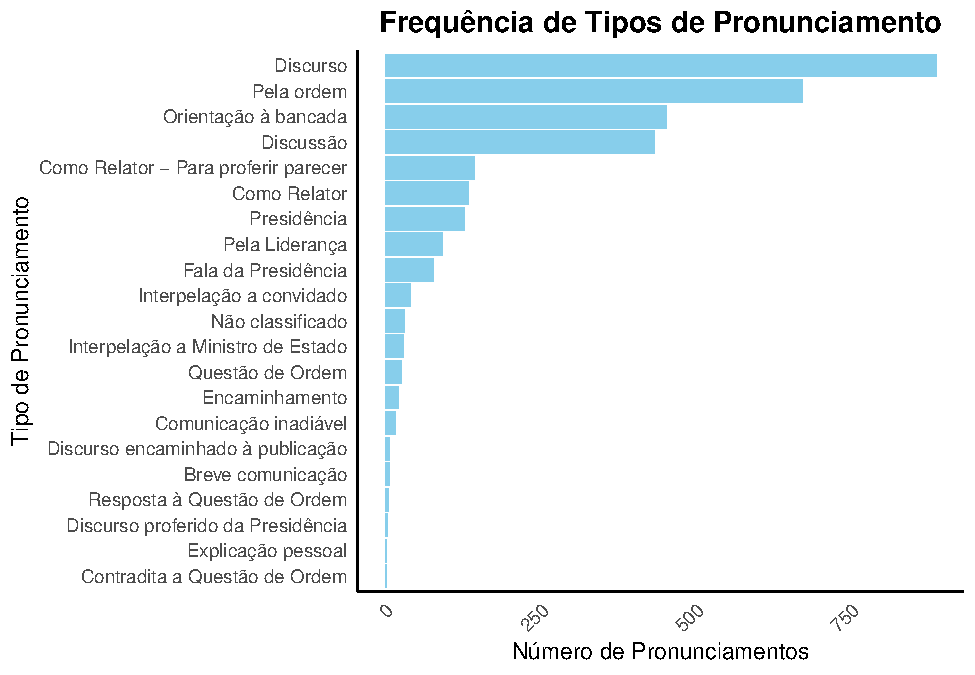
\includegraphics{Texto_files/figure-latex/unnamed-chunk-13-1.pdf}

Para fechar essa apresentação de potencialidades do pacote
concentrando-nos nos metadados a respeito dos pronunciamentos podemos
observar a distribuição de frequência do uso da palavra por partido.
Assim, figuram no ranking dos cinco principais agremiações partidárias:
PSD, MDB, PODEMOS, PT e PL.

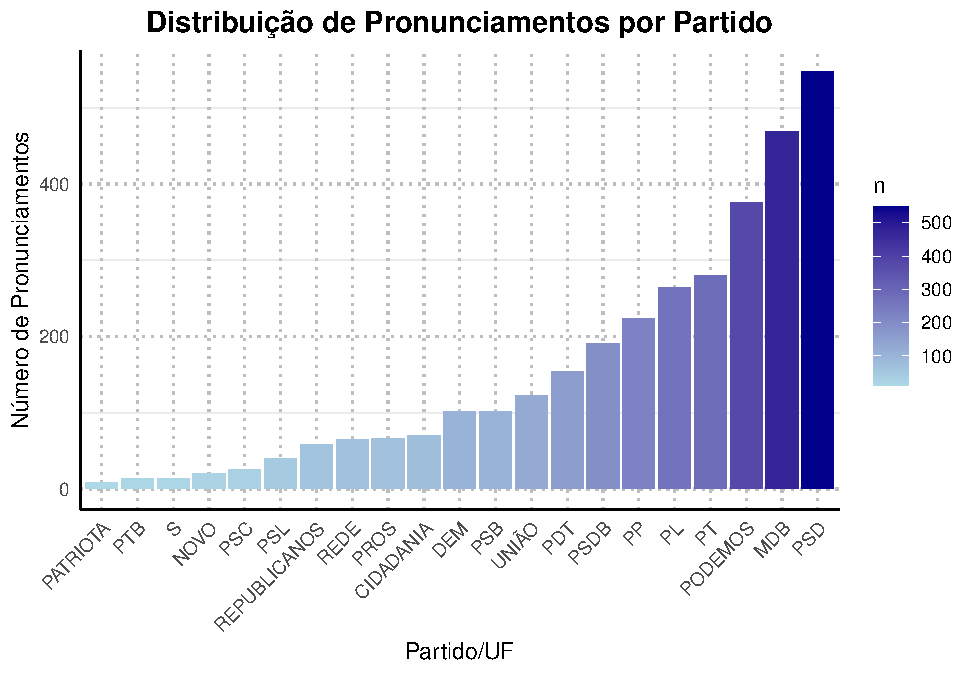
\includegraphics{Texto_files/figure-latex/unnamed-chunk-14-1.pdf}

Perceba que não mobilizamos nessa apresentação os textos dos
pronunciamentos. O que é pode ser mobilizados em execicícios de
Processamento de Linguagem Natural, no âmbito da Mineração de textos,
assim como em análises quantitativos de textos.

Com base neste estudo de caso simples, espera-se que o pesquisador possa
obter uma visão sobre o uso do pacote. Não obstante, a comunidade pode
integrar as análises técnicas de inteligência artificial (IA) e machine
learning (ML) que podem contribuir para redefinir a forma como os dados
legislativos são analisados e interpretados.

Com isso, esse conjunto de técnicas podem oferecer novas angulações para
pesquisa bem como novas perspectivas a respeito do desenvolvimento de
uma série de potenciais aplicações que podem consumir esses dados. Os
algoritmos de machine learning podem, portanto, ser mobilizados para
analisar o comportamento dos legisladores, detectar padrões de votação e
até mesmo antecipar o impacto de políticas públicas. Diante disso,
usuários podem, potencialmente, explorar padrões complexos nos dados,
identificar correlações e prever tendências (Batista, 2020; Rodrigues,
2022; Firebanks-Quevedo, 2022; Santos, 2024).

\textbf{Considerações Finais}

O pacote \emph{senatebR} é uma ferramenta para o acesso de informações
legislativas no contexto brasileiro. Com isso em mente, permite a
simplificação de obtenção de dados permitindo com que pesquisadores,
acadêmicos e profissionais realizem análises sobre diversos aspectos do
processo legislativo, do perfil dos senadores, da agenda da casa, seja
nas comissões seja no Plenário, por exemplo.

O acesso simplificado a esse conjunto de informações permite aos
pesquisadores e consultores que mais tempo seja dedicado à análise dos
dados aumentando sua capacidade analítica e consequentemente,
enriquecendo as investigações legislativas, seja na identificação de
tendências, padrões subjacentes aos dados ou até mesmo insights
significativos sobre a Câmara Alta brasileira. Isso sem mencionar, o
papel desempenhado na potencial democratização do acesso aos dados
legislativos com vistas a torná-los mais transparentes e compreensíveis,
fazendo com que o pacote promova a transparência e a accountability no
processo democrático.

Ainda, reconhecemos que a despeito do pacote representar um avanço no
acesso às informações do Senado Federal, acreditamos que ainda há espaço
para melhorias. Nessa lista de aprimoramentos, figuram: i) a expansão da
cobertura de dados seja do próprio Senado, seja como a Câmara dos
Deputados ou do Congresso Nacional. Uma vez superado esse desafio
acreditamos que essa implementação tornaria o pacote ainda mais
completo. Além disso, novos exemplos de uso são essenciais para
facilitar sua adoção e utilização por uma gama ainda mais ampla de
usuários.

Além das melhorias sugeridas anteriormente, cabe considerar considerar
potencial a integração de técnicas avançadas de inteligência artificial
(IA) e machine learning (ML) na medida em que essas tecnologias
possibilitam transformar a maneira como os dados legislativos são
analisados e interpretados, abrindo novas perspectivas de pesquisa e
desenvolvimento de aplicações. Disto decorre que, com a utilização de IA
e ML, os usuários podem explorar padrões complexos nos dados
legislativos, identificar correlações e prever tendências. Por exemplo,
algoritmos de machine learning podem ser empregados para analisar o
comportamento dos legisladores, identificar padrões de votação e até
mesmo antecipar o impacto de determinadas políticas públicas com base em
dados históricos.

Além disso, o uso de técnicas de IA e ML pode potencializar o
desenvolvimento de aplicações interativas em Shiny, por exemplo. Sendo o
Shiny uma ferramenta poderosa para criar dashboards e visualizações de
dados dinâmicos, os usuários podem explorar os dados legislativos de
forma mais intuitiva e interativa, permitindo uma compreensão mais
profunda e uma tomada de decisão mais informada.

Sobre a pluralidade de usos, por exemplo, é possível criar dashboards
que acompanhem o progresso de projetos de lei, monitorem a atuação de
parlamentares ou até mesmo simulem cenários. Em resumo, a integração de
inteligência artificial, machine learning e desenvolvimento de
aplicações em Shiny representa uma oportunidade para aprimorar ainda
mais o uso do pacote de coleta de dados do Senado Federal. Ao aproveitar
todo o potencial dessas tecnologias.

\textbf{Referências Bibliográficas}

MCDONNELL, Robert Myles; DUARTE, Guilherme Jardim; FREIRE, Danilo.
Congressbr: An R Package for Analyzing Data from Brazil's Chamber of
Deputies and Federal Senate. \textbf{Latin American Research Review}, v.
54, n.~4, p.~958-969, 2019. Disponível em:
\url{https://github.com/duarteguilherme/congressbr}

MORAIS, João Henrique de Araújo et al.~Rtabnetsp: pacote R para extração
de indicadores de saúde do estado de São Paulo. \textbf{Epidemiologia e
Serviços de Saúde}, v. 30, n.~1, p.~e2020576, 2021. Disponível:
\url{https://github.com/joaohmorais/rtabnetsp}

SALDANHA, Raphael de Freitas; BASTOS, Ronaldo Rocha; BARCELLOS,
Christovam. Microdatasus: a package for downloading and preprocessing
microdata from Brazilian Health Informatics Department (DATASUS).
\textbf{Cadernos de saude publica}, v. 35, p.~e00032419, 2019.
Disponível em: \url{https://github.com/rfsaldanha/microdatasus}

MEIRELES, F.; TORRES, M. V. . siconvr: An R package to fetch data from
Plataforma +Brasil (Siconv). 2021. Disponível em:
\url{https://github.com/meirelesff/siconvr}

MEIRELES, Fernando; SILVA, Denisson; COSTA, Beatriz. ElectionsBR: R
functions to download and clean Brazilian electoral data. 2016.
Disponível em: \url{https://github.com/silvadenisson/electionsBR}

RODRIGUES, Waldecy et al.~Uso de machine learning para a análise de
projetos legislativos de desenvolvimento regional: o caso da zona franca
de Manaus. \textbf{Informe Gepec}, v. 26, n.~2, p.~127-140, 2022.

BATISTA, Mariana. QUAIS POLÍTICAS IMPORTAM? Usando ênfases na agenda
legislativa para mensurar saliência. \textbf{Revista Brasileira de
Ciências Sociais}, v. 35, p.~e3510411, 2020.

FIREBANKS-QUEVEDO, Daniel et al.~Using machine learning to identify
incentives in forestry policy: Towards a new paradigm in policy
analysis. \textbf{Forest Policy and Economics}, v. 134, p.~102624, 2022.

VAQUEIRO, Ramon et al.~Machine Learning Applied to Open Government Data
for the Detection of Improprieties in the Application of Public
Resources. In: \textbf{Proceedings of the XIX Brazilian Symposium on
Information Systems}. 2023. p.~213-220.

OLIVEIRA, Danilo Amaral de. \textbf{Compreendendo e prevendo o processo
legislativo via ciência de dados}. 2019. Tese de Doutorado. Universidade
de São Paulo.

RUBIATTI, Bruno de Castro. Para além do plenário: o papel decisório das
comissões no Senado Federal brasileiro. \textbf{Revista de Sociologia e
Política}, v. 28, n.~75, p.~e005, 2020.

FERREIRA, Wesley Rodrigues Santos; DE CASTRO RUBIATTI, Bruno.
CARACTERIZAÇÃO DA EXPERTISE DOS SENADORES MEMBROS DA COMISSÃO DE
AGRICULTURA E REFORMA AGRÁRIA (CRA) DO SENADO FEDERAL (2005-2018).
\textbf{Novos Olhares Sociais}, v. 5, n.~2, p.~141-171, 2022.

NASCIMENTO, E. O. O sistema de comissões brasileiro: elementos para uma
agenda de pesquisa. Revista de ciência política brasileira, vol.~21,
n.~2, p.~61-72, jul./dez. 2012

SANTOS, Vinicius; LOPES, Dawisson Belém. Confirmação: o lugar do Senado
Federal na política externa brasileira da Nova República.
\textbf{Dados}, v. 66, p.~e20200243, 2022.

SANTOS, Vinicius. \emph{Inside the Fog}: Assessing Foreign Policy
Expertise in the Brazilian Federal Senate. Encontro da Associação
Brasileira de Ciência Política. 2024.

LEMOS, L. B.; RANINCHESKI, S. Carreiras políticas no Senado brasileiro:
um estudo das composições do Plenário e da Comissão de Justiça e
Cidadania na década de 1990. In: LEMOS, L. B. (Org.). O Senado Federal
brasileiro no pós-constituinte. Brasília: Senado Federal; Unilegis, 2008

RICCI, P. A produção legislativa de iniciativa parlamentar no Congresso:
diferenças e similaridades entre a Câmara dos Deputados e o Senado
Federal In: LEMOS, L. B. (Org.). O Senado Federal brasileiro no
pós-constituinte. Brasília: Senado Federal; Unilegis, 2008

RUBIATTI, B. C. Sistema de resolução de conflitos e o papel do Senado
como câmara revisora no Bicameralismo Brasileiro, Revista Brasileira de
Ciência Política, n.23, 2017, p.~35-74

SOUZA E SILVA, J. N. A. A comissão de direitos humanos e legislação
participativa (CDH) no senado brasileiro: um estudo sobre sua composição
(2005-2018). Caos -- Revista Eletrônica de Ciências Sociais, João
Pessoa, n.~23, p.~79 -112, jul./dez. 2019. Disponível em:
\url{https://periodicos.ufpb.br/ojs2/index.php/caos/index}

FIGUEIREDO FILHO, Dalson et al.~Seven reasons why: a user's guide to
transparency and reproducibility. \textbf{Brazilian Political Science
Review}, v. 13, p.~e0001, 2019.

CHRISTENSEN, Garret and SODERBERG, Courtney (2015), Manual of best
practices in transparent social science research. Berkeley: University
of California.

DA-RT, Data access and research transparency (2012), Ethics guide
changes. Available at . Accessed on February, 14, 2019

ELMAN, Colin and KAPISZEWSKI, Diana (2014). Data access and research
transparency in the qualitative tradition. PS: Political Science and
Politics. Vol. 47, Nº 01, pp.~43-47.

DUNNING, Thad and ROSENBLATT, Fernando (2016), Transparency and
reproducibility in multi-method research. Revista de Ciencia Política.
Vol. 36, Nº 03, pp.~773-783.

FREESE, Jeremy and PETERSON, David (2017), Replication in social
science. Annual Review of Sociology. Vol. 43, Nº 01, pp.~147-165.

GHERGHINA, Sergiu and KATSANIDOU, Alexia (2013), Data availability in
political science journals. European Political Science. Vol. 12,
pp.~333-349.

GLEDITSCH, Nils Petter and JANZ, Nicole (2016), Replication in
international relations. International Studies Perspectives. Vol. 17, Nº
04, pp.~361-366.

LUPIA, Arthur and ELMAN, Colin (2014), Openness in political science:
data access and research transparency. PS: Political Science \&
Politics. Vol. 47, Nº 01, pp.~19- 42.

STOCKEMER, Daniel; KOEHLER, Sebastian, and LENZ, Tobias (2018), Data
access, transparency, and replication: new insights from the political
behavior literature. PS: Political Science \& Politics. Vol. 51, Nº 04,
pp.~01-05.

WICKHAM, Hadley; BRYAN, Jennifer. \textbf{R packages}. O'Reilly Media,
Inc, 2023.

WICKHAM, Hadley; ÇETINKAYA-RUNDEL, Mine; GROLEMUND, Garrett. \textbf{R
for data science}. O'Reilly Media, Inc., 2023.

WICKHAM, Hadley. \textbf{Advanced r}. Chapman and Hall/CRC, 2019.

WEINSTEIN, Jeremey; GOLDSTEIN, Joshua. The Benefits of a Big Tent:
Opening up Government in Developing Countries: A Response to Yu \&
Robinson's the New Ambiguity of Open Government. \textbf{UCLA L.
Rev.~Discourse}, v. 60, p.~38, 2012.

CLARKE, Amanda; FRANCOLI, Mary. What's in a name? A comparison of 'open
government'definitions across seven open government partnership members.
\textbf{JeDEM-eJournal of eDemocracy and Open Government}, v. 6, n.~3,
p.~248-266, 2014.

SANDOVAL-ALMAZAN, Rodrigo; GIL-GARCIA, J. Ramon. Towards an evaluation
model for open government: A preliminary proposal. In:
\textbf{Electronic Government: 13th IFIP WG 8.5 International
Conference, EGOV 2014, Dublin, Ireland, September 1-3, 2014. Proceedings
13}. Springer Berlin Heidelberg, 2014. p.~47-58.

ABU-SHANAB, Emad A. Reengineering the open government concept: An
empirical support for a proposed model. \textbf{Government Information
Quarterly}, v. 32, n.~4, p.~453-463, 2015.

DE BLASIO, Emiliana; SORICE, Michele. Open Government: a tool for
democracy?. \textbf{Media Studies}, v. 7, n.~14, 2016.

KORNBERGER, Martin et al.~When bureaucracy meets the crowd: Studying
``open government'' in the Vienna City Administration.
\textbf{Organization Studies}, v. 38, n.~2, p.~179-200, 2017.

\bibliographystyle{unsrt}
\bibliography{references.bib}


\end{document}
